\chapter[The End - Ideas and Final Remarks]{The End - Ideas and Final Remarks}\label{chap:the_end}
% LINGO: unorthodox.
In the last chapter of this thesis, I would like to present some ideas for future research in persuasive password support. Although I would have loved to start working on these already now, they go beyond the scope of this thesis and should be left to future work. As final remarks, I want to share my views on current developments of password authentication, where I see it in the near future, and how its future can be shaped more positively. 

\section{Ideas for Future Work}
The recommendations in Section \ref{sec:summary:recommendations} touched on future work on a high level. However, one recommendation was to follow up on ideas off the beaten path. Addressing this criterion, the following sections provide more specific ideas to work on password support in the future. 

%-- be frank and say we don't want to create ``recommendations'' or ``guidelines'', because it takes years and more diverse samples to solidify such. Therefore, we think it's better to show ``ideas'' what this can mean and where the topic is going. 

%TODO keep in mind: relate all ideas to the P4P framework. 
\subsection{Follow-Up Studies} 
% combine PASDJO and Personality study.
First and foremost, it will be worthwhile to address the limitations of the studies we conducted, or follow up on the leads from initial results. For instance, the PASDJO deployment in the wild suffered from lack of demographic data to understand individual differences in password perception. The second study on personality lacked more randomness of the available passwords and it would thus be straightforward solution to integrate a short, optional psychometric questionnaire into PASDJO. Alternatively, we could have crowd-workers fill out a more elaborate psychometric survey before they play PASDJO and then fit regression models on the data. In any case, by combining the two approaches we will overcome current limitations of the two studies at once. 

% of course the password reuse manager. 
Furthermore, it will be vital to evaluate the Password Reuse Manager (PWRM, see Chapter \ref{chap:perdespassup}) with a longitudinal study. At this point, we used a rapid iterative design method that was focused on qualitative feedback on features. The next step will be to invite a larger audience to test it for at least one month. To boost usage numbers during the field trial, the browser extension can be made compatible with additional browsers with very little effort. It is already built on the WebExtensions API, which is increasingly solid on all major browsers. We had also identified specific research questions that can be answered with A/B testing. One of the issues was that users kept their previous password managers activated and the additional extension simply generated more effort. The follow-up study should therefore screen for participants who do not use a password manager yet (group A), and another group who will be required to move over to the PWRM as single management solution throughout the entire study (group B). To extend the method space (see recommendation \ref{recommendation:method_space} in Section \ref{sec:summary:recommendations}) and better understand how the support works for the users, the study should conclude with the \textit{break up-/love-letter method}\footurl{https://medialabamsterdam.com/toolkit/method-card/break-uplove-letter/}{28.03.2018}. Here, participants decide whether to write a love or a break-up letter to the PWRM, which will allow us to understand the emotional component of password support. 

% in-situ
Finally, some of our other studies involved a password \textit{creation} task (see Chapters \ref{chap:pws_and_personality},\ref{chap:decoy}, and \ref{chap:emojipasswords}). Although we followed guidelines to establish realistic scenarios, we would have been desirable to study password selection in-situ. Thus, in the future, we should leverage existing web-applications to test concepts when they are mature enough. Establishing collaborations with industry partners is critical to carry out this research approach. 

\subsection{Personalizing Password Policies}\label{sec:pst:personalizing-policies}
Personalization is a current big trend in user experience design and persuasive technology\footurl{https://www.forbes.com/sites/shephyken/2017/05/13/recommended-just-for-you-the-power-of-personalization/}{28.03.2018}, especially since the breakthrough in machine-learning capabilities. It was already an element in the Persuasive Authentication Framework \cite{Forget2007PersuasionEducationSecurity}. We have found that personality has a notable influence on how users perceive password policies (see Chapter \ref{chap:pws_and_personality}). Therefore, it is conceivable to leverage state-of-the-art computing power to tailor password requirements to individual users instead of relying on a one-fits-all approach. Hypothetically, if the system could detect what policy will \textit{help} the user to find the best trade-off between password strength and usability the user experience of using the system would not be degraded by password authentication (as it is now). I provided initial pointers about the benefits in a position paper adjunct to \textit{PERSUASIVE'17} \cite{Seitz2017PersonalizingPasswordPolicies}. 

Tackling this challenge is possible with several focus areas, where the P4P framework can guide design decisions. For instance, we could advance algorithms to detect re-used passwords more reliably at registration. Khern-am-nuai \etal have showed an initial proof-of-concept that keystroke dynamics provide useful features \cite{Khern-am-nuai2017Journal}, but the analysis was done post-hoc. Machine-learning can potentially enable reuse detection already at enrollment and allow us to tailor feedback more appropriately. For instance, we can design a solution that makes alternatives to password reuse more salient, in case reuse generates considerable risks (process depicted in Figure \ref{fig:summary:flow-chart}). Similar approaches are conceivable with different personality profiles. However, here it is much more likely to tailor personalize support strategies during password \textit{reset}, because the service potentially possesses more data about the user at that point. 
%TODO: argumentation ist noch nicht ganz geradlinig. 

\begin{figure}
	\centering
	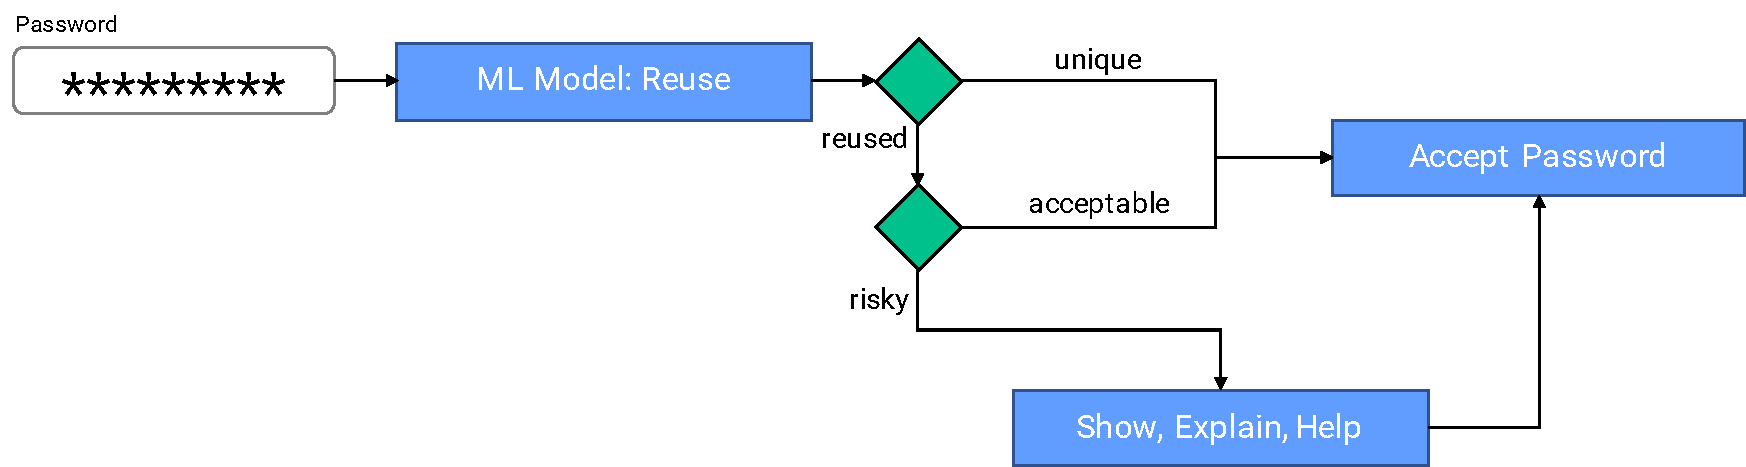
\includegraphics[width=\linewidth]{figures/summary/flow-chart}
	\caption{Personalized intervention for password reuse. The keystrokes inside a password field are analyzed by a machine learning model. If the password is unique, do not intervene. If the password is reused, but there are no signs for overlaps between categories, we can accept the password, too. However, if the password is reused across different categories, we use the show-explain-help paradigm to empower users to make an informed decision. In any case, the password is accepted to avoid being too restrictive. }
	\label{fig:summary:flow-chart}
\end{figure}

 
%Segreti \etal SOUPS 2017
%\cite{Seitz2017PersonalizingPasswordPolicies}
%\cite{Segreti2017AdaptivePolicies}

%\subsection{Keystrokes as Reuse Heuristics}
%Reuse is the worst. We should design a persuasive strategy that shows alternatives to reused passwords. As a first step, we need to detect that the password a user just entered has been reused on other websites. Since this is not bad per se, we also need to check how strong it is, and how likey it is a ``throw away'' password that users don't care about anyway. -- elaborate on this. Show an updated flow chart from CHI EA 


\subsection{Contextualizing Password Feedback}

like \cite{Kroeze2012GamifyingAuthentication} Pokémon Go could use an evolving Pokemon as password strength feedback. 

``wuerstel meter'' as an example that we implemented.

minimizes habituation effects as mentioned by Ur \etal \cite{Ur2012HelpingUsersCreateBetterPasswords}.

\subsection{What do other people do? Clichés and biased views of password selection strategies}
people are biased to think that their password strategy is unique, i.e. they do not realize that other users behave similarly. it would be interesting to study the revelation process - ask people on the street how they think that others create their passwords for different categories. independent variables: who creates a password, for what context?

social patterns helpful: Instead of saying a password is better than 90\% of other \textit{users} we could frame it as ``this password lowers your chance of being attacked by XX percent'' or ``this password is better than 90\% of passwords used on the internet''. issues: it's kind of hard to really be truthful here. deceptive in some ways and that's not something we want. 

\subsection{Password Audits After Third Party Breaches}

if a data leak is made public, sites can use the leaked passwords to audit the users on their sites. if they find that passwords have been compromised, they should decide (depending on a matching user name) if the password on their site should be invalidated and the user prompted to update it.

kind of resembles a post-hoc blacklist.  

catch: carefully craft Password Reset Emails \cite{Kim2017TooBusy}

risks: users could be confused, looks like a phishing attack (why was my account hacked?)

feature for password meters to determine stringency: 
there could be a framework that uses \url{https://haveibeenpwned.com/API/v2} to adjust stringency 

from \cite{Bishop1995ProactivePasswordChecking}: ``Many sites have responded to this threat with a reactive solution -- they scan their own password files and advise those users whose passwords they are able to crack. The problem with this solution is that while the local site is testing its security, the password file is still vulnerable from the outside. The other problems, of course, are that the testing is very time-consuming and only reports on those passwords it is able to crack. It does nothing to address user passwords which fall outside of the specific test cases (e.g., it is possible for a user to use as a password the letters ``query'' if this combination is not in the in-house test dictionary, it will not be detected, but there is nothing to stop an outside cracker from having a more sophisticated dictionary!).''

\subsection{Helping to Make Sense of a Breach}
how does user behavior change after a breach? not much says Huh \etal \cite{Huh2017TooBusy}. But it would be interesting to correlate other factors with altered behavior: do different personality traits influence how a user ``cleans up the mess'' after a breach?


\section{Final Thoughts}
Lorem Epson. 

\begin{figure}[htpb]
	\centering
	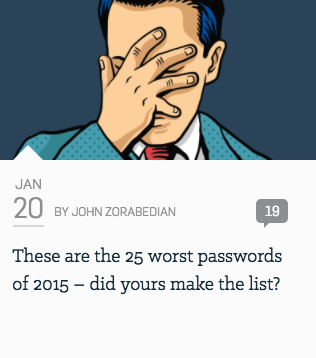
\includegraphics[width=0.3\linewidth]{shaming/nakedsecurity-sophos}
	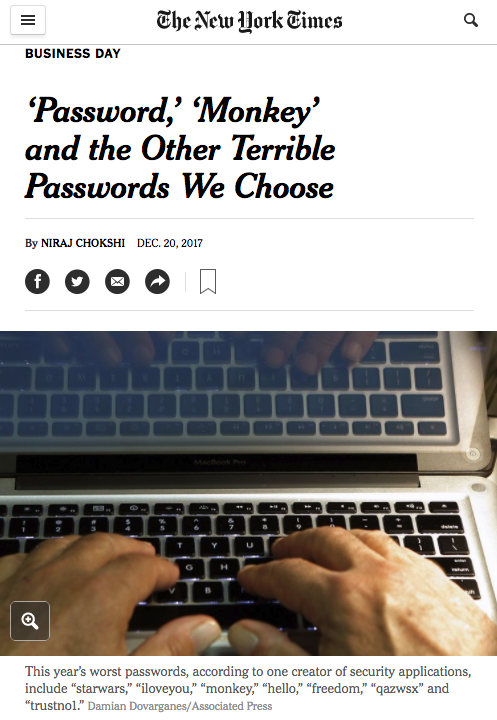
\includegraphics[width=0.3\linewidth]{shaming/nytimes}
	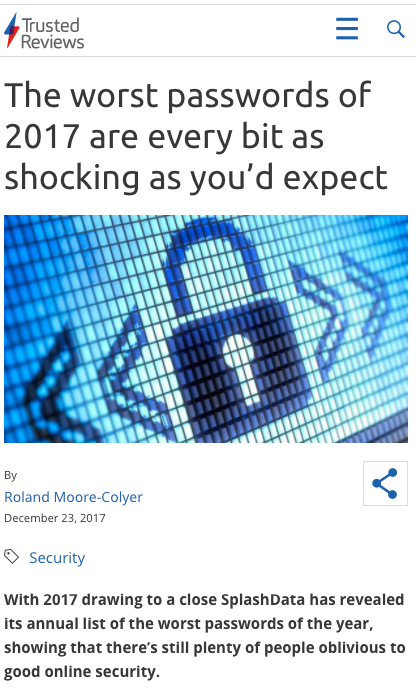
\includegraphics[width=0.3\linewidth]{shaming/trusted-reviews}
\end{figure}

Key thoughts

\begin{itemize}
\item Passwords are bad. Let's hope passwords vanish at some point. Make machines intelligent enough to decide if a user should be granted access or not. But this brings new problems.
\item Maybe passwords are the vinyl records of usable security - everyone agrees that it's kind of an obsolete technology but there's something to it that ensure they don't disappear. %TODO come up with a better analogy.
 \item  if passwords become obsolete tomorrow, many of us will not grief. 
 \item  the media should stop shaming the users 
 \item  it's okay to forget passwords! reference to the article Franziska shared with me (SZ,  01.12.2017 ``Die Kunst zu vergessen'' \footurl{http://www.sueddeutsche.de/wissen/neurowissenschaft-die-kunst-zu-vergessen-1.3772438}{02.01.2018}.)
 \item 	ad networks for webpages can undermine any attempt to secure one's account. Too many websites show ads that can run harmful scripts. yes, adblockers do prevent this, but not everyone has one installed (especially novice users don't). Frightening research on this: \footurl{https://freedom-to-tinker.com/2017/12/27/no-boundaries-for-user-identities-web-trackers-exploit-browser-login-managers/}{02.01.2018}
\end{itemize}

It's interesting that often the same idea pops up every other year. so although there are no replication studies, evaluating the same idea multiple times with different setups and specifics, kind of goes in that direction. 

%TODO: take the ``pws are not going away'' section and put it here?


%TODO I have more thann 100 ``takeaways'' from papers. This could be a funny ``sermon'' too (Luther's 100 theses);